%\section{Background}
This section provides a background on two main topics of the project: Recurrent Neural Networks (RNN) and Machine Translation (MT). We begin by looking into neural networks and why RNNs are well suited for MT. Then, we will look into some of the historical and current approaches for machine translation.

\section{Neural Networks}
\cite{rojas2013neural} define neural networks as ``distributed, adaptive, generally nonlinear learning  machines built from many different processing elements''. They can approximate a function by learning the input-output mapping. Neural networks like feed-forward multi-layer perceptrons, shown in Figure \ref{mlp}, can approximate any (continuous) function to an arbitrary accuracy if the number of hidden neurons are large enough \citep{hornik1989multilayer}. These networks can be trained using the backpropogation algorithm \citep{rumelhart1988learning} by updating the weights and biases based on an objective function. As the training progresses, the network updates its weights in a way that its predicted output moves closer to the ground truth\footnote{ground truth - reference output provided by direct observation as opposed to inference}. A one layer feed-forward neural network can be written as follows:


%of the network to match the predicted output to the labelled output
\begin{equation}
NN_{MLP1} (x) = g(xW^1 + b^1 )W^2 + b^2
\end{equation}

where g is any non linear activation function, $x$ is an input vector, $W^1, W^2, b^1$ and  $b^2$ are the weights and biases for the network.

Unlike other machine learning approaches where input features have to be hand-engineered, neural networks can learn the required features from the training data. 

\begin{figure}[ht]
	\centering
	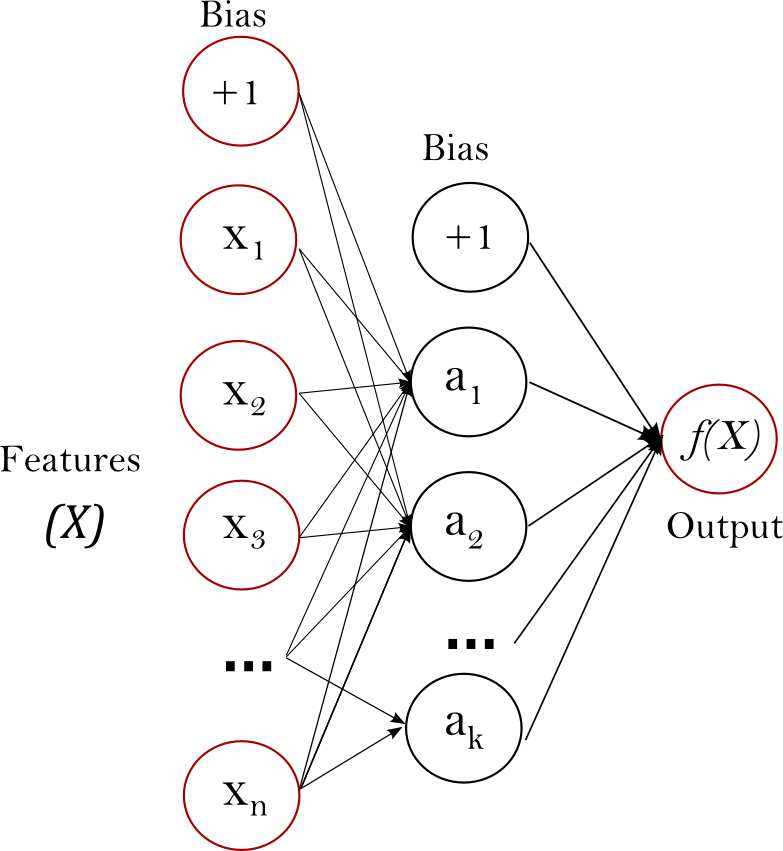
\includegraphics{images/multilayerperceptron_network}
	\caption{Multilayer perceptron network with one hidden layer. Figure taken from  \cite{pedregosa2011scikit}}
	\label{mlp}.
\end{figure}

One class of neural network model called Recurrent Nerual Network (RNN) \citep{elman1990finding} is particularly well suited for machine translation. In natural languages, the input is a sequence of words of arbitrary length based on some structure properties of the language. RNNs allow for representing an input sequence of arbitrary length as fixed-sized vectors based on its structural properties. A simple RNN \citep{goldberg2016primer} can be defined as follows.

\begin{align}
h_{1:n},  y_{1:n} &= RNN(h_0,x_{1:n}) \\
h_i &= R(h_{i-1},x_i;\theta) \\
y_i &= O(h_i;\theta)
\end{align}
\[ 
x_i \in \mathbb{R}^{d_{in}}, y_i \in \mathbb{R}^{d_{out}}, h_i \in \mathbb{R}^{f({d_{out}})} \]

where $x_{1:n}$ is the input vector, $y_{1:n}$ is the output vector and $h_{i}$ is the state vector at time-step $i$. $R$ is a non linear function applied over current input $x_i$ and previous hidden state $s_{i-1}$. $O$ is an additional function applied over the current hidden state to generate output vector.  Parameters $\theta$ are shared across the network. A simple RNN uses $sigmoid$ or $tanh$ as the non linear function in the neural units. Special kinds of neural units like Long Short-Term Memory (LSTM) \citep{hochreiter1997long} or Gated Recurrent Units (GRU) \citep{cho2014learning} can also be used. A graphical representation of the same network is shown in Figure \ref{rnn}


\begin{figure}[ht]
	\centering
	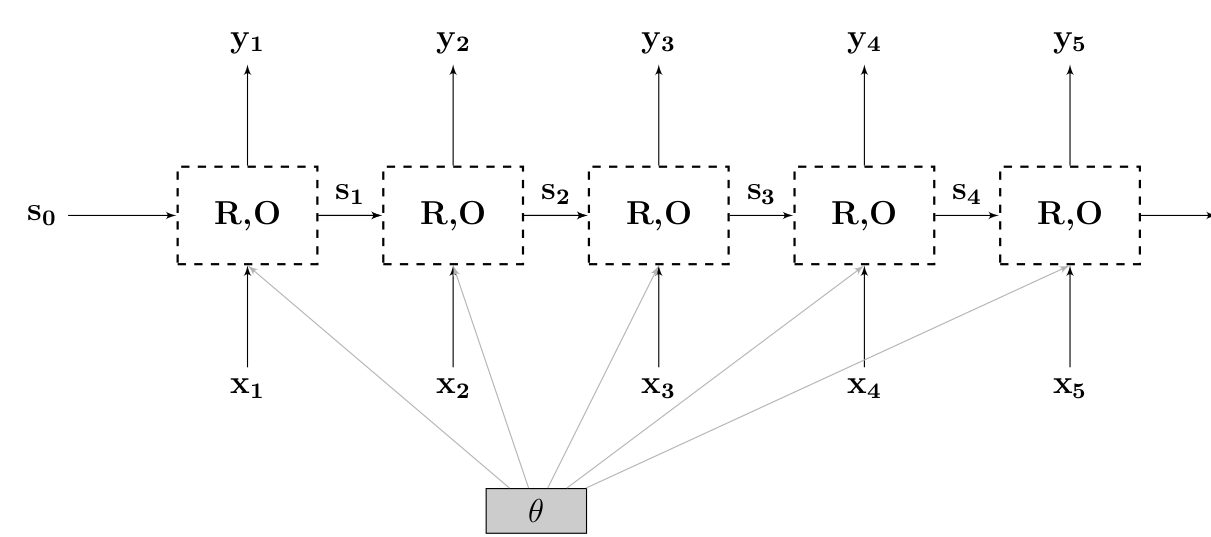
\includegraphics[scale=0.3]{images/rnn}
	\caption{Graphical representation of RNN. Figure taken from \cite{goldberg2016primer}}.
	\label{rnn}
\end{figure}


The input for these neural networks is a sequence of vectors not words. NMT systems use word embeddings to represent input words. It is a way of representing words in a vocabulary as vectors in a higher dimensional space. These representations have been good at capturing semantic and syntactic regularities in languages \citep{mikolov2013distributed}. When used as input, these models have also been shown to improve the performance of many NLP systems in tasks such as \textit{MT} \citep{vaswani2017attention, sennrich2015neural}, \textit{sentiment classification} \citep{kumar2016ask}, and \textit{part of speech tagging} \citep{kumar2016ask}. The vector representation for words in these models primarily depend their co-occurrence count with other words within a window size. These vectors capture syntactic, semantic and morphological properties of the words. 

%\begin{figure}[ht]
%	\centering
%	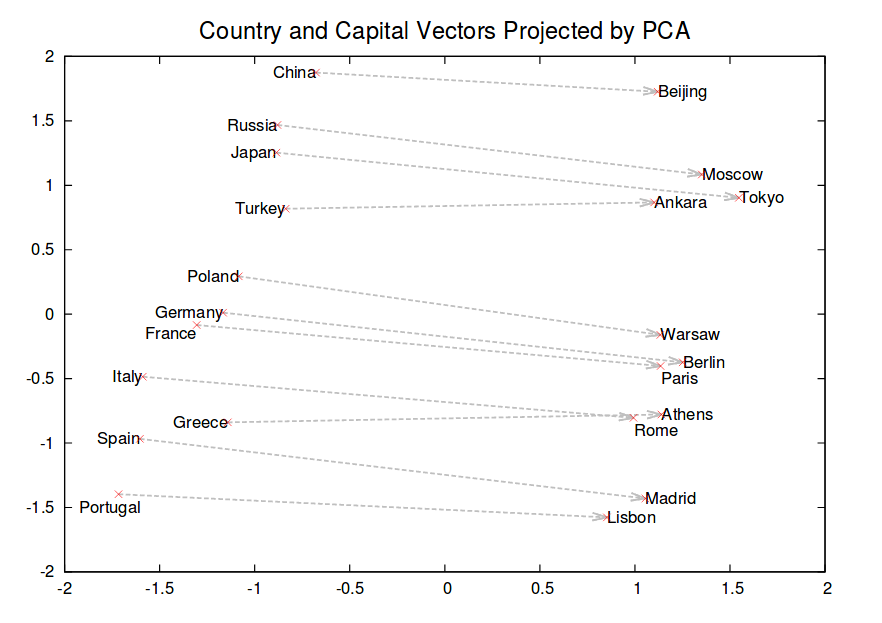
\includegraphics[scale=0.5]{images/embeddings}
%	\caption{Two-dimensional Principal component analysis (PCA) projection of 1000-dimensional vectors of countries and their capitals \citep{mikolov2013distributed}}.
%	\label{embeddings}
%\end{figure}


%\footnote{Principal component analysis (PCA is dimensionality technique used here to show high dimensional vectors in 2-dimensional space.)}

One of the major challenges for many embedding models is their inability to handle Out Of Vocabulary (OOV) words.  This problem is more pronounced in languages with rich morphology. A word in morphologically rich languages encodes more information (such as gender, number, tense) as compared to morphologically poor languages which rely on word order and context. Recently, many models have been proposed to solve this problem. \cite{sun2016inside} proposed a method to integrate both external contexts and internal morphemes\footnote{Morphemes are the smallest meaningful units in a language.} to learn better word embeddings especially for rare and unknown words. \cite{bojanowski2016enriching} incorporate subword information like character n-grams\footnote{A character n-gram is a sequence of n characters from a word} for learning word embeddings during training. Overall, character embedding models, where vector representations for every character or character n-grams are learned, have be shown to generate good word embeddings for rare and unknown words. 

%%Most of these models were originally developed in English - a language with strict word order and relatively poor morphology. These models perform the best in English. 
%

%
%
%Despite their advantages, NMT systems are not capable of translating rare and unknown words. In this project, I am implementing an end to end encoder-decoder system for machine translation and an unsupervised method to handle unknown and rare words.
%

\section{Statistical Machine Translation}
Machine translation is a task of translating a source language sentence $F$ to the target language sentence $E$ using computing resources. It can effectively remove language barriers between humans, allowing assimilation of content from different languages. This potential of MT has led to substantial amount of research since the advent of digital computing. There have been many approaches to the problem such as rule-based MT, phrase-based MT, NMT, etc. In the early days, rule based approaches that used dictionaries, grammar and pre-defined rules to translate text were explored until the ALPAC report in 1966 \citep{national1966language}. The ALPAC report showed that post-editing machine translation was not cheaper or faster than human translation. 

%\subsubsection{Statistical Machine Translation}

In the late 1980s, following the success of statistical method on speech recognition, IBM research \citep{brown1993mathematics} modelled the problem of translation as a statistical optimization problem. Many SMT approaches such as word-based models \citep{brown1993mathematics}, phrase-based models \citep{koehn2003statistical,marcu2002phrase}, hierarchical phrase-based  models \citep{chiang2007hierarchical} and syntax based models \cite{galley2004s,galley2006scalable} were proposed. The goal of all the SMT systems is to maximize the probability of target sentence $f$ given the source language sentence $e$

\begin{equation}
\underset{f}{argmax \  } P(f|e) = \underset{f}{arg max } (P(f) \times P(e|f)) 
\end{equation}


where $P(f)$ is a language model and $P(e|f)$ is a translation model. Language model and translation model are sub-components of SMT systems. Language models learn to assign probability to a sequence of words in a language. They assign higher probability to sentences that are more likely to occur in the language and hence a measure of fluency in the language. Language modelling is central to many tasks in NLP including MT.  

Translation models learn the mapping between source and target language words or phrases. They measure word level translation accuracy between source and target sentences. These models were built by analyzing  monolingual, bilingual corpus and learning their probability distribution. The rise of digital text resources like parallel corpora and an increase in computing power and storage, fuelled the growth of SMT systems. Although SMT systems are robust to noisy data,  they required fine tuning for many components such as language model, reordering model, and translation model for each language pairs. They also require large amount of data and do not handle long range dependencies well.


\section{Neural Machine Translation}

An NMT system is a neural network that models the conditional probability $p(y|x)$ of generating a target language $y$ sentence given the source language sentence $x$. Generally, any NMT system consists of two components i) an \textit{encoder} that computes a sentence representation vector from the source sentence, and ii) a \textit{decoder} that transforms the vector representation to a target language sentence. RNNs are a common choice of network for both encoders and decoders as they process input in a sequential fashion. Convolution neural networks have also been used especially as an encoder \citep{kalchbrenner2013recurrent}.

%In 2003, \cite{bengio2003neural} proposed probabilistic language model based on neural networks which laid the foundation for the use of neural networks in machine translation. 

Initially, neural networks were used as a component in phrase based systems to score the quality of translation \citep{schwenk2012continuous} and to provide additional features to SMT systems \citep{zou2013bilingual}. \cite{kalchbrenner2013recurrent} proposed the first end to end approach for NMT using convolution neural networks as the encoder and RNN as the decoder. Their network suffered from the problem of vanishing gradients where the network was unable to capture long range dependencies. To overcome this problem, more sophisticated activation functions such as LSTM \citep{hochreiter1997long} or GRU \citep{cho2014learning} are used.  \cite{sutskever2014sequence} and \cite{cho2014learning} demonstrated that these gated units can handle long range dependencies better than a simple RNN \citep{elman1990finding}. An encoder-decoder network with LSTM RNNs is shown in Figure \ref{seq2seq}. The boxes in the figure are LSTM RNN units. Mathematically, an LSTM RNN unit is defined in \cite{goldberg2016primer} as follows:

\begin{align}
s_j = R_{LSTM}(s_{j-1}, x_j) &= [c_j:h_j] \\
c_j &= c_{j-1} \odot f + g \odot i \\
h_j &= tanh(c_j) \odot o \\
i &= \sigma(x_j W^{xi} + h_{j-1} W^{hi})\\
f &= \sigma(x_j W^{xf} + h_{j-1} W^{hf})\\
o &= \sigma(x_j W^{xo} + h_{j-1} W^{ho})\\
g &= tanh(x_j W^{xg} + h_{j-1}W^{hg})\\
y_j &= O_{LSTM}(s_j)
\end{align}
\[ 
s_i \in \mathbb{R}^{2 \cdot d_{h}}, x_i \in \mathbb{R}^{d_{x}}, [c_j, h_j, i, f, o, g] \in \mathbb{R}^{{d_{h}}}, W^{xo} \in \mathbb{R}^{d_x x d_h}, W^{ho} \in \mathbb{R}^{d_h x d_h}  \]

where $x_j$, $y_j$ and $h_j$ are the input vector, output vector and the hidden vector repectively. $\odot$ is component-wise product. $i$, $f$ and $o$ are input, forget and output gates respectively. $g$ is the update candidate.

\begin{figure}[ht]
	\centering
	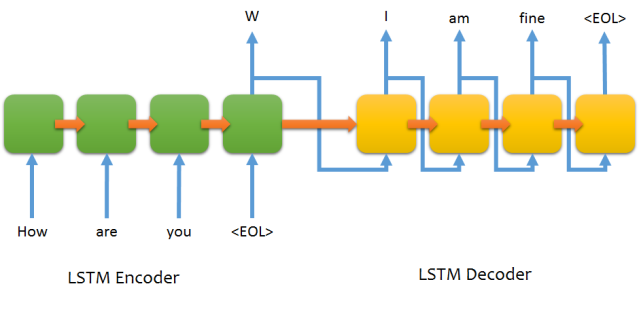
\includegraphics[scale=0.9]{images/seq2seq}
	\caption{RNN with LSTM encoder and decoder. Figure taken from \cite{farizrahman4u}}.
	\label{seq2seq}
\end{figure}


\subsubsection{Attention based Encoder-Decoder models}

These simple encoder-decoder networks summarize the source sentence in a fixed length context vector. \cite{bahdanau2014neural} noted that these networks were inadequate to represent long sentences due to the fixed dimension of the context vector. While this problem could theoretically be solved by increasing the dimension of the context vector, the computing power and memory required to train such a network sets an upper limit even today.

\cite{bahdanau2014neural} proposed an attention based encoder-decoder architecture to mitigate this problem.  This allowed for the encoder to produce better sentence representation for longer sentences which in turn improved the translation quality. In their additive approach, a single feed forward neural networks that can learn to assign different weights to the hidden layer vectors was used. These weighted sum of the hidden layer vectors $h_{1:n}$ called context vector $c_i$ is calculated each time decoder generates a new word as shown in Figure \ref{attention}.

\begin{align}
c_i &= \sum_{j=1}^{n} \alpha_{ij} h_j \\
\alpha_{ij} &= \frac{\hat{a}_{ij}}{\sum_j \hat{a}_{ij}}\\
\hat{a}_{ij} &= att(s_i, h_j)
\end{align}


%\cite{bahdanau2014neural} proposed an attention based encoder-decoder architecture which is capable of learning word alignment between source and target sentences.In their additive approach, a single feed forward neural networks that can learn to assign different weights to the hidden layer vectors was used. 


where $att(s_i, h_j)$ is an attention function that calculates the weights for each encoder hidden state $h_{1:n}$, for a given decoder state $s_i$. They also used bi-directional RNN which reads the sentence from both directions. The state vector from both direction right to left  $\overleftarrow{h_j}$ and left to right $\overrightarrow{h_j}$ is concatenated for each word. The attention mechanism is applied over this concatenated hidden state vector $h_j = [\overleftarrow{h_j};\overrightarrow{h_j}]$. The whole network is trained with negative log-likelihood as the objective function using stochastic gradient descent.


\begin{figure}[ht]
	\centering
	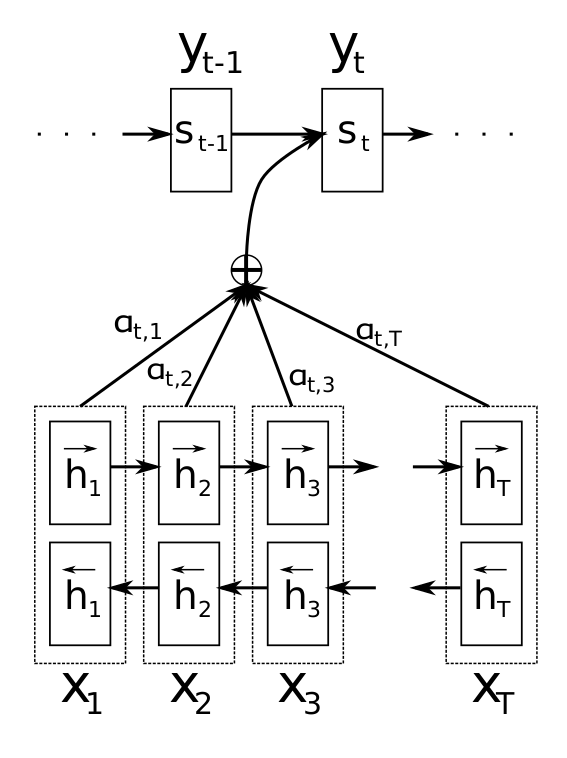
\includegraphics[scale=0.35]{images/attention}
	\caption{Attention based encoder. Figure taken from \cite{bahdanau2014neural}}.
	\label{attention}
\end{figure}


%\begin{align}
%a_t(s) = align(h_t, \bar h_s)  = \dfrac{exp(score(h_t, \bar h_s))}{\sum_{s'} exp(score(h_t, \bar h_{s'}))}
%\end{align}

\cite{luong2015effective} proposed two simpler but effective variations of attention mechanism namely: 1) a global attention model where all words in the source sentence are attended, and 2) a local attention model where only a subset of the source words are attended at a time. In the global attention mechanism, which is very similar to one proposed in \cite{bahdanau2014neural}, they did away with bi-directional, concatenated state vector $h_j = [\overleftarrow{h_j};\overrightarrow{h_j}]$. They simplified the computation path to make it run faster. Their model produced state-of-the-art results in WMT'14 and WMT'15 for English to German translation. 


In this project, we use the global attention based encoder-decoder model proposed in \cite{luong2015effective} as the baseline NMT system for evaluation. The models discussed so far cannot handle words that are not in their vocabulary. In the next chapter, we will look at some of techniques that allow us to handle OOV words.




% Basics needed to understand the rest of the text with references to authoritative literature sources

%
%
%
%
%In their model, the source language sentence will be encoded into a real valued vector using the encoder. The decoder will decode the vector to a target language sentence to produce the output. 
%
%Unlike, SMT systems, NMT systems generalize well, do not require domain knowledge and are more tolerant to noisy data \cite{bibid}. 
%
%
%NMT systems use vector representation, also called word embeddings, for input words and internal states. Word embedding is a way of representing words in the vocabulary using vectors in a high dimensional space.Word embedding models like \cite{bengio2003neural,mikolov2013distributed,pennington2014glove} etc., learn word representation in continuous vector space where similar words are expected to occur closer to each other. These models have been successfully used in many NLP tasks like Machine Translation. The vector representation for word in most of these models primarily depend on word co-occurrence or context words within a window size capturing syntactic, semantic and morphological properties of natural languages. 
%
%
%%Most of these models were originally developed in English - a language with strict word order and relatively poor morphology. These models perform the best in English. 
%
%One of the major challenges for many embedding models is their inability to handle out of vocabulary words.  This problem is more pronounced in languages with rich morphology. A word in morphologically rich languages encodes more information (such as gender, number, tense) as compared to morphologically poor languages which rely on word order and context. 
%
%
%Despite their advantages, NMT systems are not capable of translating rare and unknown words. In this project, I am implementing an end to end encoder-decoder system for machine translation and an unsupervised method to handle unknown and rare words.
%






%In 2003, \cite{bengio2003neural} proposed a language model developed using neural network.
%
%Data Sparcity Problem.
